\subsubsubsection{CreateActivity Function}

\begin{enumerate}

\item Profile

\begin{enumerate}

\item Description

The CreateActivity function is used to create Activity object Id based on given Agreement by the Requestor Node. 
It uses the POST /activity method. The Activity is created in New state.
%This call shall get routed as a provider event.

\item Side

Requestor

\end{enumerate}

\item Request

\begin{enumerate}

\item Input

\begin{tcolorbox}[boxrule=0pt, frame empty]
\begin{verbatim}

timeout

\end{verbatim}
\end{tcolorbox}

Object

\begin{tcolorbox}[boxrule=0pt, frame empty]
\begin{verbatim}

agreementId

\end{verbatim}
\end{tcolorbox}

\begin{table}[H]
\footnotesize

\begin{center}
\begin{tabular}{|p{3cm}|l|p{3cm}|p{3cm}|p{4cm}|} 
\hline
\rowcolor{lightgray}	Name	& MO.	& Type	& Example & 	Description \\
\hline

agreementId				& M	& 	string				&								&	Agreement Identifier \\ 
\hline

timeout					& O	& 	number(\$float)		&	5							&	Timeout used in blocking calls waiting for eg. acknowledgement. 
																						How many seconds server should wait for response/acknowledgement of an action 
																						(0.0 means it should wait for other party's response indefinitely) \\ 
\hline

%paymentDueDate			& M &	string(\$date-time)	&	YYYY-MM-DDThh:mm:ss.sssZ	&	Payment Due Date \\
%\hline

\end{tabular}
\end{center}
\end{table}


\item REST Method

\begin{tcolorbox}[boxrule=0pt, frame empty]
\begin{verbatim} 

POST /activity

\end{verbatim}
\end{tcolorbox}

\end{enumerate}

\item Response

\begin{table}[H]
\footnotesize

\begin{center}
\begin{tabular}{|c|l|} 
\hline
\rowcolor{lightgray}	Code 		& 	Description \\
\hline
201	 		&	Success \\
\hline
400			&	(400) Bad request \\
\hline
403			&	(403) Forbidden	\\
\hline
404			&	(404) The specified resource was not found. \\
\hline
500			&	(500) Server error. \\
\hline
\end{tabular}
\end{center}
\end{table}

\item Result

\begin{tcolorbox}[boxrule=0pt, frame empty]
\begin{verbatim}

activityId

\end{verbatim}
\end{tcolorbox}

\begin{table}[H]
\footnotesize

\begin{center}
\begin{tabular}{|p{3cm}|l|p{3cm}|p{3cm}|p{4cm}|} 
\hline
\rowcolor{lightgray}	Name	& MO.	& Type	& Example & 	Description \\
\hline

activityId				&	&	string				&																		&	Activity Identifier \\
\hline   

\end{tabular}
\end{center}
\end{table}

\item Workflow

(Please see Figure ~\ref{fig:RCA} on page ~\pageref{fig:RCA}):

\begin{figure}[H]
    \centering
    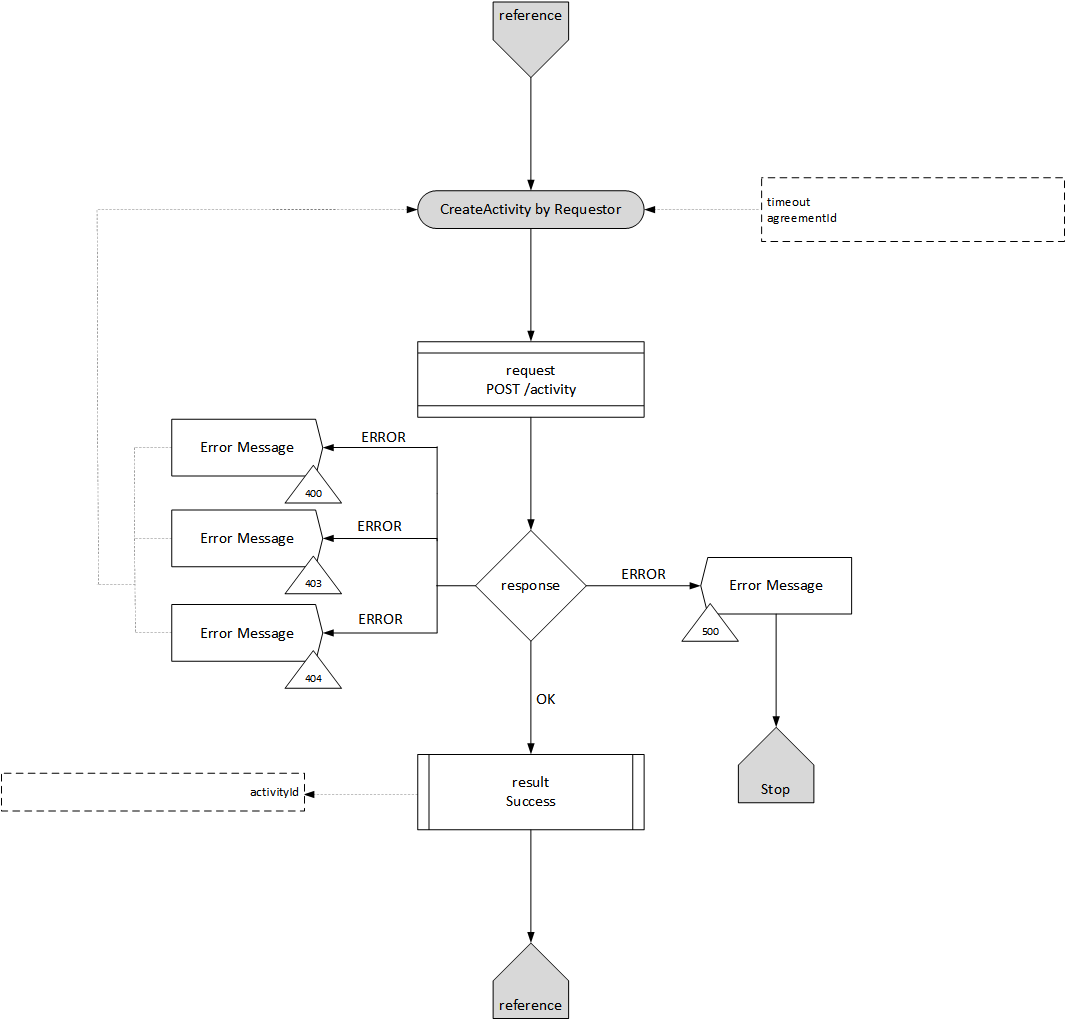
\includegraphics[width=12cm,height=12cm,angle=0]{./diag/Workflow/Activity/CreateActivity-R-Workflow.png}
    \caption{Requestor Workflow Create Activity }
	\label{fig:RCA}
\end{figure}


\end{enumerate}

\newpage

%%% Exec 
\subsubsubsection{Exec Function}

\begin{enumerate}

\item Profile

\begin{enumerate}

\item Description

The Exec function is used to execute a set of ExeScript commands in the context of created Activity object. 
This function is used by the Requestor Node.
It uses the POST /activity/\{activityId\}/exec method. 
%This call shall get routed directly to ExeUnit.

\item Side

Requestor

\end{enumerate}

\item Request

\begin{enumerate}

\item Input

\begin{tcolorbox}[boxrule=0pt, frame empty]
\begin{verbatim}

activityId

\end{verbatim}
\end{tcolorbox}

Object

\begin{tcolorbox}[boxrule=0pt, frame empty]
\begin{verbatim}

{
  "text": "string"
}

\end{verbatim}
\end{tcolorbox}

\begin{table}[H]
\footnotesize

\begin{center}
\begin{tabular}{|p{3cm}|l|p{3cm}|p{3cm}|p{4cm}|} 
\hline
\rowcolor{lightgray}	Name	& MO.	& Type	& Example & 	Description \\
\hline

activityId				& M	& 	string				&			&	Activity Identifier \\ 
\hline

ExeScript				& M	& 	json(commands)		&	DEPLOY, START, RUN, SUSSPEND, RESUME, TRANSFER	&	 \\ 
\hline

%paymentDueDate			& M &	string(\$date-time)	&	YYYY-MM-DDThh:mm:ss.sssZ	&	Payment Due Date \\
%\hline

\end{tabular}
\end{center}
\end{table}


\item REST Method

\begin{tcolorbox}[boxrule=0pt, frame empty]
\begin{verbatim} 

POST /activity/{activityId}/exec

\end{verbatim}
\end{tcolorbox}

\end{enumerate}

\item Response

\begin{table}[H]
\footnotesize

\begin{center}
\begin{tabular}{|c|l|} 
\hline
\rowcolor{lightgray}	Code 		& 	Description \\
\hline
200	 		&	Success \\
\hline
400			&	(400) Bad request \\
\hline
403			&	(403) Forbidden	\\
\hline
404			&	(404) The specified resource was not found. \\
\hline
500			&	(500) Server error. \\
\hline
\end{tabular}
\end{center}
\end{table}

\item Result

\begin{tcolorbox}[boxrule=0pt, frame empty]
\begin{verbatim}

"\"batchId\""

\end{verbatim}
\end{tcolorbox}

\begin{table}[H]
\footnotesize

\begin{center}
\begin{tabular}{|p{3cm}|l|p{3cm}|p{3cm}|p{4cm}|} 
\hline
\rowcolor{lightgray}	Name	& MO.	& Type	& Example & 	Description \\
\hline

batchId				&	&	string				&			&	Batch Identifier \\
\hline   

\end{tabular}
\end{center}
\end{table}

\item Workflow

(Please see Figure ~\ref{fig:RBE} on page ~\pageref{fig:RBE}):

\begin{figure}[H]
    \centering
    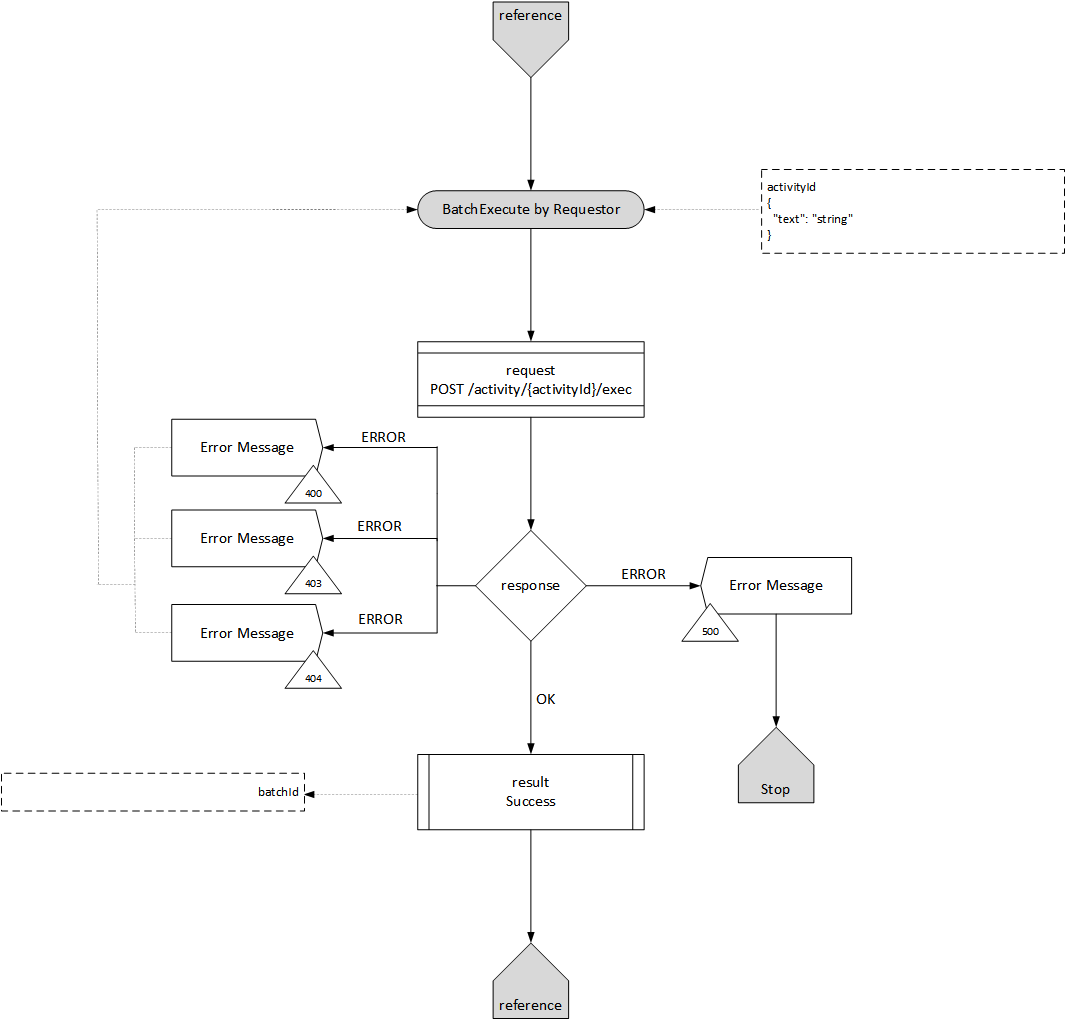
\includegraphics[width=12cm,height=12cm,angle=0]{./diag/Workflow/Activity/BatchExecute-R-Workflow.png}
    \caption{Requestor Workflow Batch Execute }
	\label{fig:RBE}
\end{figure}


\end{enumerate}

\newpage

%%% GetExecBatchResult
\subsubsubsection{GetExecBatchResult Function}

\begin{enumerate}

\item Profile

\begin{enumerate}

\item Description

The GetExecBatchResult function is used to collect the result sets returned while ExeScript batch in executing. 
This function is used by the Requestor Node.
It uses the GET /activity/\{activityId\}/exec/\{batchId\} method. 
%This call shall get routed directly to ExeUnit.

\item Side

Requestor

\end{enumerate}

\item Request

\begin{enumerate}

\item Input

\begin{tcolorbox}[boxrule=0pt, frame empty]
\begin{verbatim}

activityId
batchId
commandIndex
timeout

\end{verbatim}
\end{tcolorbox}


%Object
%\begin{tcolorbox}[boxrule=0pt, frame empty]
%\begin{verbatim}
%{
%  "text": "string"
%}
%\end{verbatim}
%\end{tcolorbox}

\begin{table}[H]
\footnotesize

\begin{center}
\begin{tabular}{|p{3cm}|l|p{3cm}|p{3cm}|p{4cm}|} 
\hline
\rowcolor{lightgray}	Name	& MO.	& Type	& Example & 	Description \\
\hline

activityId				& M	& 	string				&			&	Activity Identifier \\ 
\hline

batchId					& M	& 	string				&			&	Batch Identifier \\ 
\hline

commandIndex			& O	& 	number(\$integer)	&			&	Wait until command with the specified index finishes. 
																	Must be accompanied by a valid "pollTimeout" query parameter. \\ 
\hline

timeout					& O	& 	number(\$float)		&	5		&	Timeout used in long-polling calls (in seconds). 
																	How many seconds server should wait for response containing new events 
																	(0.0 means it should return immediately if there are no events) \\ 
\hline

%paymentDueDate			& M &	string(\$date-time)	&	YYYY-MM-DDThh:mm:ss.sssZ	&	Payment Due Date \\
%\hline

\end{tabular}
\end{center}
\end{table}


\item REST Method

\begin{tcolorbox}[boxrule=0pt, frame empty]
\begin{verbatim} 

GET /activity/{activityId}/exec/{batchId}

\end{verbatim}
\end{tcolorbox}

\end{enumerate}

\item Response

\begin{table}[H]
\footnotesize

\begin{center}
\begin{tabular}{|c|l|} 
\hline
\rowcolor{lightgray}	Code 		& 	Description \\
\hline
200	 		&	Success \\
\hline
400			&	(400) Bad request \\
\hline
403			&	(403) Forbidden	\\
\hline
404			&	(404) The specified resource was not found. \\
\hline
500			&	(500) Server error. \\
\hline
\end{tabular}
\end{center}
\end{table}

\item Result

\begin{tcolorbox}[boxrule=0pt, frame empty]
\begin{verbatim}

[
  {
    "index": 0,
    "eventDate": "YYYY-MM-DDThh:mm:ss.sssZ",
    "result": "Ok",
    "stdout": "string",
    "stderr": "string",
    "message": "string",
    "isBatchFinished": true
  }
]

\end{verbatim}
\end{tcolorbox}

\begin{table}[H]
\footnotesize

\begin{center}
\begin{tabular}{|p{3cm}|l|p{3cm}|p{3cm}|p{4cm}|} 
\hline
\rowcolor{lightgray}	Name	& MO.	& Type	& Example & 	Description \\
\hline

index				&	&	number(\$integer)	&			&	Batch Identifier \\
\hline   

eventDate			&  &	string(\$date-time)	&	YYYY-MM-DDThh:mm:ss.sssZ	&	Event Date \\
\hline

result				&	&	string	&	[Ok, ...]	&	Result \\
\hline

stdout				&	&	string	&			&	STDOUT \\
\hline

stderr				&	&	string	&			&	STDERR \\
\hline

message				&	&	string	&			&	Message \\
\hline

isBatchFinished		&	&	boolean	& [true, false]	&	 \\
\hline

\end{tabular}
\end{center}
\end{table}

\item Workflow

(Please see Figure ~\ref{fig:RGEBR} on page ~\pageref{fig:RGEBR}):

\begin{figure}[H]
    \centering
    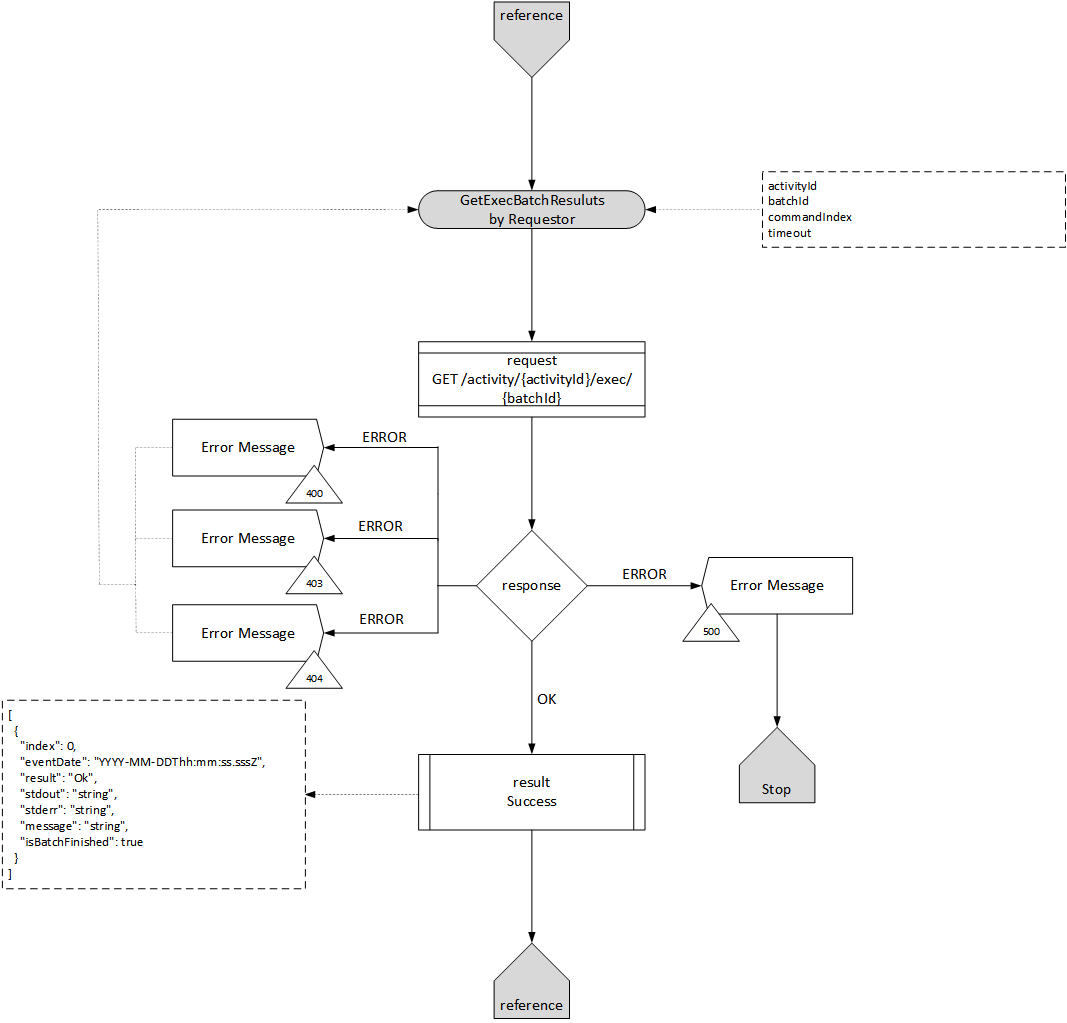
\includegraphics[width=12cm,height=12cm,angle=0]{./diag/Workflow/Activity/GetExecBatchResults-R-Workflow.png}
    \caption{Requestor Workflow Get Execute Batch Results}
	\label{fig:RGEBR}
\end{figure}


\end{enumerate}

\newpage

%% Destroy

\subsubsubsection{DestroyActivity Function}

\begin{enumerate}

\item Profile

\begin{enumerate}

\item Description

The DestroyActivity function is used to destroy given Activity.  
It uses the DELETE /activity/\{activityId\} method. 
%This call shall get routed as a provider event.

\item Side

Requestor

\end{enumerate}

\item Request

\begin{enumerate}

\item Input

\begin{tcolorbox}[boxrule=0pt, frame empty]
\begin{verbatim}

activityId
timeout

\end{verbatim}
\end{tcolorbox}

%Object

%\begin{tcolorbox}[boxrule=0pt, frame empty]
%\begin{verbatim}

%agreementId

%\end{verbatim}
%\end{tcolorbox}

\begin{table}[H]
\footnotesize

\begin{center}
\begin{tabular}{|p{3cm}|l|p{3cm}|p{3cm}|p{4cm}|} 
\hline
\rowcolor{lightgray}	Name	& MO.	& Type	& Example & 	Description \\
\hline

activityId				& M	& 	string				&								&	Activity Identifier \\ 
\hline

timeout					& O	& 	number(\$float)		&	5							&	Timeout used in blocking calls waiting for eg. acknowledgement. 
																						How many seconds server should wait for response/acknowledgement of an action 
																						(0.0 means it should wait for other party's response indefinitely) \\ 
\hline

%paymentDueDate			& M &	string(\$date-time)	&	YYYY-MM-DDThh:mm:ss.sssZ	&	Payment Due Date \\
%\hline

\end{tabular}
\end{center}
\end{table}


\item REST Method

\begin{tcolorbox}[boxrule=0pt, frame empty]
\begin{verbatim} 

DELETE /activity/{activityId}

\end{verbatim}
\end{tcolorbox}

\end{enumerate}

\item Response

\begin{table}[H]
\footnotesize

\begin{center}
\begin{tabular}{|c|l|} 
\hline
\rowcolor{lightgray}	Code 		& 	Description \\
\hline
200	 		&	Success \\
\hline
403			&	(403) Forbidden	\\
\hline
404			&	(404) The specified resource was not found. \\
\hline
500			&	(500) Server error. \\
\hline
\end{tabular}
\end{center}
\end{table}

\item Result

\begin{tcolorbox}[boxrule=0pt, frame empty]
\begin{verbatim}

as above

\end{verbatim}
\end{tcolorbox}

%\begin{table}[H]
%\footnotesize
%\begin{center}
%\begin{tabular}{|p{3cm}|l|p{3cm}|p{3cm}|p{4cm}|} 
%\hline
%\rowcolor{lightgray}	Name	& MO.	& Type	& Example & 	Description \\
%\hline
%activityId				&	&	string		&	&	Activity Identifier \\
%\hline   
%\end{tabular}
%\end{center}
%\end{table}

\item Workflow

(Please see Figure ~\ref{fig:RDA} on page ~\pageref{fig:RDA}):

\begin{figure}[H]
    \centering
    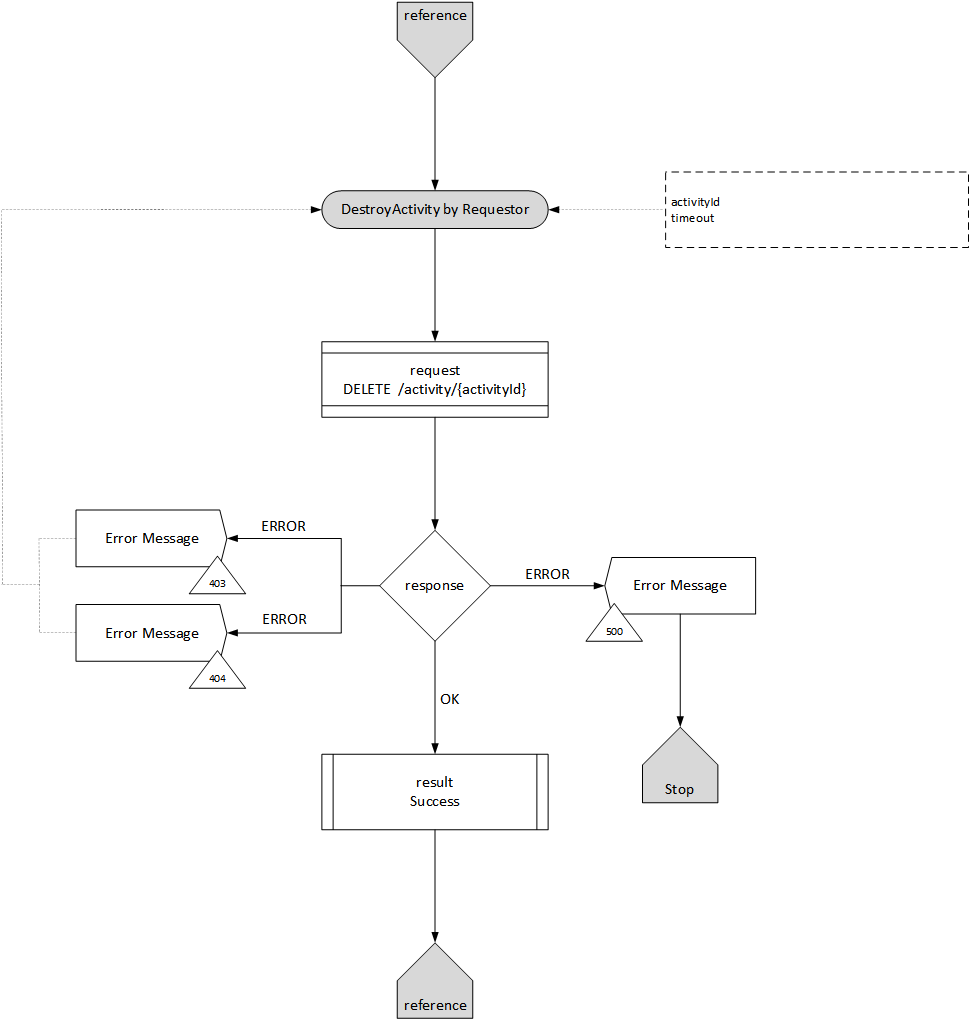
\includegraphics[width=12cm,height=12cm,angle=0]{./diag/Workflow/Activity/DestroyActivity-R-Workflow.png}
    \caption{Requestor Workflow Destroy Activity }
	\label{fig:RDA}
\end{figure}


\end{enumerate}

\newpage

%% ActivityAgreement

\subsubsubsection{CheckActivityAgreement Function}

\begin{enumerate}

\item Profile

\begin{enumerate}

\item Description

The CheckActivityAgreement function is used to return agreementId coresponding to the activity.  
It uses the GET /activity/\{activityId\}/agreement method. 

\item Side

Both

\end{enumerate}

\item Request

\begin{enumerate}

\item Input

\begin{tcolorbox}[boxrule=0pt, frame empty]
\begin{verbatim}

activityId

\end{verbatim}
\end{tcolorbox}

%Object

%\begin{tcolorbox}[boxrule=0pt, frame empty]
%\begin{verbatim}

%agreementId

%\end{verbatim}
%\end{tcolorbox}

\begin{table}[H]
\footnotesize

\begin{center}
\begin{tabular}{|p{3cm}|l|p{3cm}|p{3cm}|p{4cm}|} 
\hline
\rowcolor{lightgray}	Name	& MO.	& Type	& Example & 	Description \\
\hline

activityId				& M	& 	string				&								&	Activity Identifier \\ 
\hline

%paymentDueDate			& M &	string(\$date-time)	&	YYYY-MM-DDThh:mm:ss.sssZ	&	Payment Due Date \\
%\hline

\end{tabular}
\end{center}
\end{table}


\item REST Method

\begin{tcolorbox}[boxrule=0pt, frame empty]
\begin{verbatim} 

GET /activity/{activityId}/agreement

\end{verbatim}
\end{tcolorbox}

\end{enumerate}

\item Response

\begin{table}[H]
\footnotesize

\begin{center}
\begin{tabular}{|c|l|} 
\hline
\rowcolor{lightgray}	Code 		& 	Description \\
\hline
200	 		&	Agreement \\
\hline
403			&	(403) Forbidden	\\
\hline
404			&	(404) The specified resource was not found. \\
\hline
500			&	(500) Server error. \\
\hline
\end{tabular}
\end{center}
\end{table}

\item Result

\begin{tcolorbox}[boxrule=0pt, frame empty]
\begin{verbatim}

agreementId

\end{verbatim}
\end{tcolorbox}

\begin{table}[H]
\footnotesize
\begin{center}
\begin{tabular}{|p{3cm}|l|p{3cm}|p{3cm}|p{4cm}|} 
\hline
\rowcolor{lightgray}	Name	& MO.	& Type	& Example & 	Description \\
\hline
agreementId				&	&	string		&	&	Agreement Identifier \\
\hline   
\end{tabular}
\end{center}
\end{table}

\item Workflow

(Please see Figure ~\ref{fig:BCAA} on page ~\pageref{fig:BCAA}):

\begin{figure}[H]
    \centering
    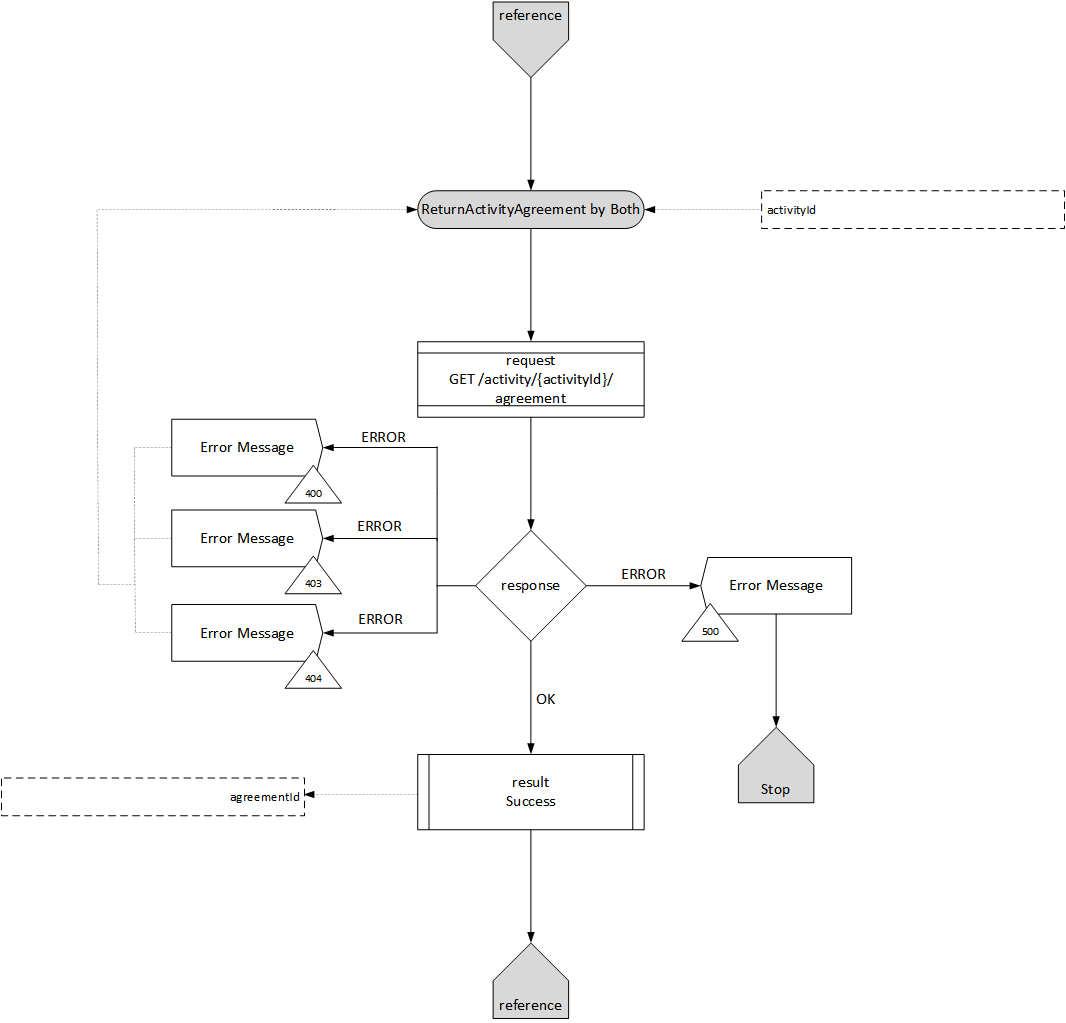
\includegraphics[width=12cm,height=12cm,angle=0]{./diag/Workflow/Activity/ReturnActivityAgreement-B-Workflow.png}
    \caption{Both Workflow Check Activity Agreement }
	\label{fig:BCAA}
\end{figure}


\end{enumerate}

\newpage


%% GetState

\subsubsubsection{GetState Function}

\begin{enumerate}

\item Profile

\begin{enumerate}

\item Description

The GetState function is used to return state coresponding to the activity.  
It uses the GET /activity/\{activityId\}/state method. 

\item Side

Both

\end{enumerate}

\item Request

\begin{enumerate}

\item Input

\begin{tcolorbox}[boxrule=0pt, frame empty]
\begin{verbatim}

activityId

\end{verbatim}
\end{tcolorbox}

%Object

%\begin{tcolorbox}[boxrule=0pt, frame empty]
%\begin{verbatim}

%agreementId

%\end{verbatim}
%\end{tcolorbox}

\begin{table}[H]
\footnotesize

\begin{center}
\begin{tabular}{|p{3cm}|l|p{3cm}|p{3cm}|p{4cm}|} 
\hline
\rowcolor{lightgray}	Name	& MO.	& Type	& Example & 	Description \\
\hline

activityId				& M	& 	string				&								&	Activity Identifier \\ 
\hline

%paymentDueDate			& M &	string(\$date-time)	&	YYYY-MM-DDThh:mm:ss.sssZ	&	Payment Due Date \\
%\hline

\end{tabular}
\end{center}
\end{table}


\item REST Method

\begin{tcolorbox}[boxrule=0pt, frame empty]
\begin{verbatim} 

GET /activity/{activityId}/state

\end{verbatim}
\end{tcolorbox}

\end{enumerate}

\item Response

\begin{table}[H]
\footnotesize

\begin{center}
\begin{tabular}{|c|l|} 
\hline
\rowcolor{lightgray}	Code 		& 	Description \\
\hline
200	 		&	Success \\
\hline
404			&	(404) The specified resource was not found. \\
\hline
500			&	(500) Server error. \\
\hline
\end{tabular}
\end{center}
\end{table}

\item Result

\begin{tcolorbox}[boxrule=0pt, frame empty]
\begin{verbatim}

{
  "state": [
    "New"
  ],
  "reason": "string",
  "errorMessage": "string"
}

\end{verbatim}
\end{tcolorbox}

\begin{table}[H]
\footnotesize
\begin{center}
\begin{tabular}{|p{3cm}|l|p{3cm}|p{3cm}|p{4cm}|} 
\hline
\rowcolor{lightgray}	Name	& MO.	& Type	& Example & 	Description \\
\hline

state				&	&	string(enum)		& [New, Initialized, Deployed, Ready, Unresponsive, Terminated]	&	State pair tuple (CurrentState, NextState). 
																													NextState is equal to null if there is no pending transition between states.\\
\hline  

reason 				&	&	string		&		& Reason for Activity termination \\
\hline

errorMessage		&	&	string		&		& If error caused state change - error message shall be provided. \\
\hline
 
\end{tabular}
\end{center}
\end{table}

\item Workflow

(Please see Figure ~\ref{fig:BGS} on page ~\pageref{fig:BGS}):

\begin{figure}[H]
    \centering
    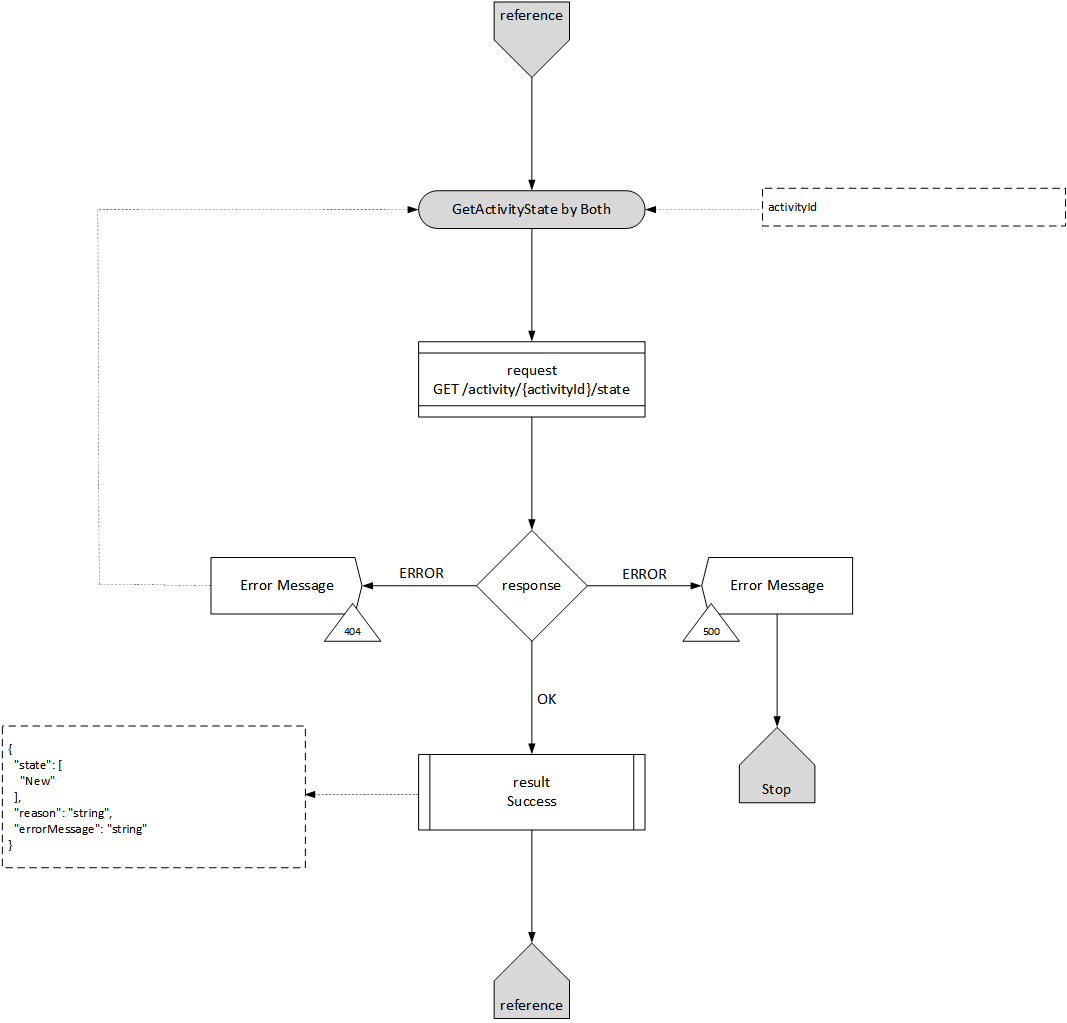
\includegraphics[width=12cm,height=12cm,angle=0]{./diag/Workflow/Activity/GetActivityState-B-Workflow.png}
    \caption{Both Workflow Get Activity State }
	\label{fig:BGS}
\end{figure}


\end{enumerate}

\newpage

%% GetCurrentUsage

\subsubsubsection{GetCurrentUsage Function}

\begin{enumerate}

\item Profile

\begin{enumerate}

\item Description

The GetCurrentUsage function is used to return usage coresponding to the activity.  
It uses the GET /activity/\{activityId\}/usage method. 

\item Side

Both

\end{enumerate}

\item Request

\begin{enumerate}

\item Input

\begin{tcolorbox}[boxrule=0pt, frame empty]
\begin{verbatim}

activityId

\end{verbatim}
\end{tcolorbox}

%Object

%\begin{tcolorbox}[boxrule=0pt, frame empty]
%\begin{verbatim}

%agreementId

%\end{verbatim}
%\end{tcolorbox}

\begin{table}[H]
\footnotesize

\begin{center}
\begin{tabular}{|p{3cm}|l|p{3cm}|p{3cm}|p{4cm}|} 
\hline
\rowcolor{lightgray}	Name	& MO.	& Type	& Example & 	Description \\
\hline

activityId				& M	& 	string				&								&	Activity Identifier \\ 
\hline

%paymentDueDate			& M &	string(\$date-time)	&	YYYY-MM-DDThh:mm:ss.sssZ	&	Payment Due Date \\
%\hline

\end{tabular}
\end{center}
\end{table}


\item REST Method

\begin{tcolorbox}[boxrule=0pt, frame empty]
\begin{verbatim} 

GET /activity/{activityId}/usage

\end{verbatim}
\end{tcolorbox}

\end{enumerate}

\item Response

\begin{table}[H]
\footnotesize

\begin{center}
\begin{tabular}{|c|l|} 
\hline
\rowcolor{lightgray}	Code 		& 	Description \\
\hline
200	 		&	Success \\
\hline
404			&	(404) The specified resource was not found. \\
\hline
500			&	(500) Server error. \\
\hline
\end{tabular}
\end{center}
\end{table}

\item Result

\begin{tcolorbox}[boxrule=0pt, frame empty]
\begin{verbatim}

{
  "currentUsage": [
    123.5,
    34000
  ],
  "timestamp": 0
}

\end{verbatim}
\end{tcolorbox}

\begin{table}[H]
\footnotesize
\begin{center}
\begin{tabular}{|p{3cm}|l|p{3cm}|p{3cm}|p{4cm}|} 
\hline
\rowcolor{lightgray}	Name	& MO.	& Type	& Example & 	Description \\
\hline

currentUsage		&	&	number(\$double)		& [123.5, 34000]	&	Current vector of usage counters consumed by the Activity. 
																			The sequence of values corresponds to Usage Vector property 
																			(golem.usage.vector) as indicated in the Agreement (Offer part).\\
\hline  

timestamp			&	&	integer	&	0	&	Usage update timestamp (UTC) \\
\hline
 
\end{tabular}
\end{center}
\end{table}

\item Workflow

(Please see Figure ~\ref{fig:BGAU} on page ~\pageref{fig:BGAU}):

\begin{figure}[H]
    \centering
    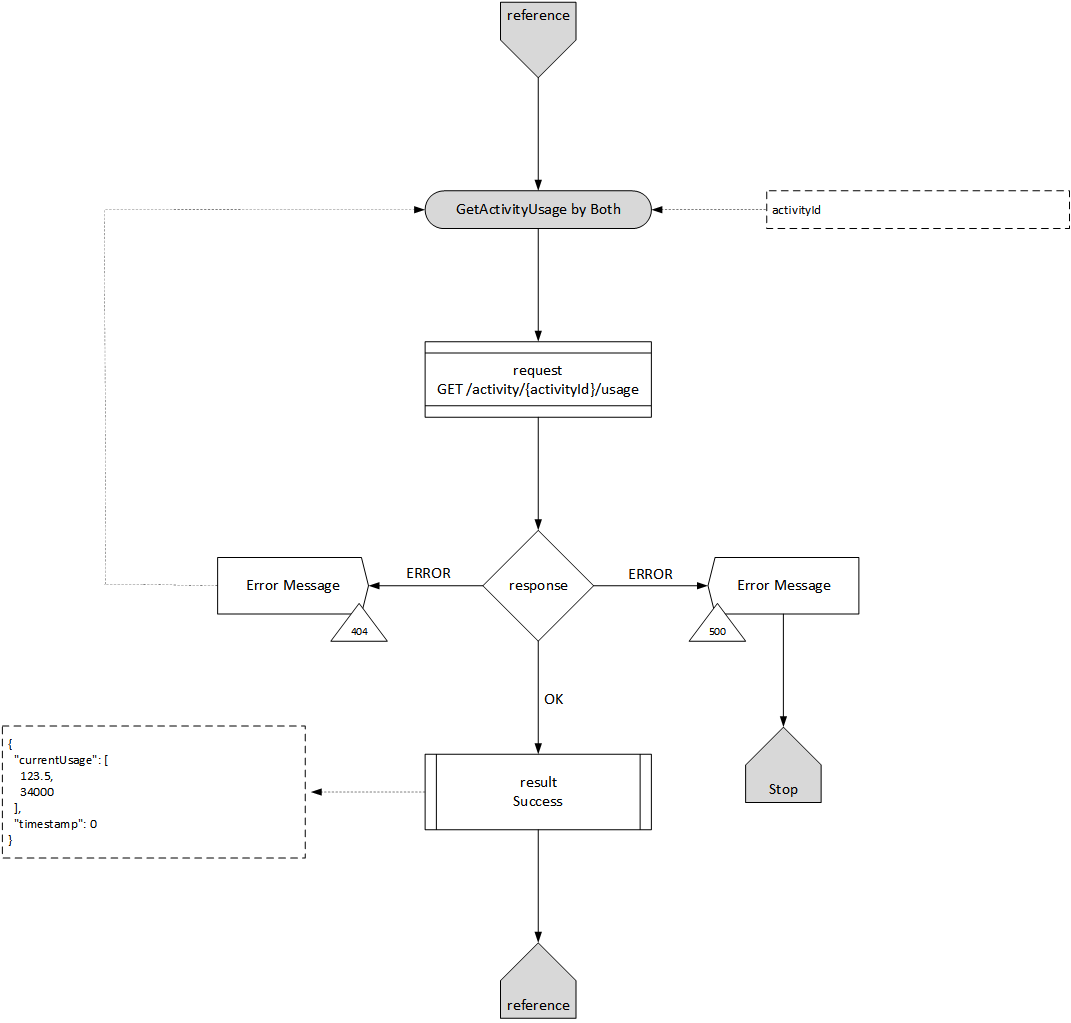
\includegraphics[width=12cm,height=12cm,angle=0]{./diag/Workflow/Activity/GetActivityUsage-B-Workflow.png}
    \caption{Both Workflow Get Activity Usage }
	\label{fig:BGAU}
\end{figure}


\end{enumerate}

\newpage

%% GetRunningCommand

\subsubsubsection{GetRunningCommand Function}

\begin{enumerate}

\item Profile

\begin{enumerate}

\item Description

The GetRunningCommand function is used to return the ExeScript command coresponding to the activity.  
It uses the GET /activity/\{activityId\}/command method. 

\item Side

Requestor

\end{enumerate}

\item Request

\begin{enumerate}

\item Input

\begin{tcolorbox}[boxrule=0pt, frame empty]
\begin{verbatim}

activityId

\end{verbatim}
\end{tcolorbox}

%Object

%\begin{tcolorbox}[boxrule=0pt, frame empty]
%\begin{verbatim}

%agreementId

%\end{verbatim}
%\end{tcolorbox}

\begin{table}[H]
\footnotesize

\begin{center}
\begin{tabular}{|p{3cm}|l|p{3cm}|p{3cm}|p{4cm}|} 
\hline
\rowcolor{lightgray}	Name	& MO.	& Type	& Example & 	Description \\
\hline

activityId				& M	& 	string				&								&	Activity Identifier \\ 
\hline

%paymentDueDate			& M &	string(\$date-time)	&	YYYY-MM-DDThh:mm:ss.sssZ	&	Payment Due Date \\
%\hline

\end{tabular}
\end{center}
\end{table}


\item REST Method

\begin{tcolorbox}[boxrule=0pt, frame empty]
\begin{verbatim} 

GET /activity/{activityId}/command

\end{verbatim}
\end{tcolorbox}

\end{enumerate}

\item Response

\begin{table}[H]
\footnotesize

\begin{center}
\begin{tabular}{|c|l|} 
\hline
\rowcolor{lightgray}	Code 		& 	Description \\
\hline
200	 		&	Success \\
\hline
404			&	(404) The specified resource was not found. \\
\hline
500			&	(500) Server error. \\
\hline
\end{tabular}
\end{center}
\end{table}

\item Result

\begin{tcolorbox}[boxrule=0pt, frame empty]
\begin{verbatim}

[
  {
    "batchId": "string",
    "command": "string",
    "progress": "string",
    "params": [
      "string"
    ]
  }
]

\end{verbatim}
\end{tcolorbox}

\begin{table}[H]
\footnotesize
\begin{center}
\begin{tabular}{|p{3cm}|l|p{3cm}|p{3cm}|p{4cm}|} 
\hline
\rowcolor{lightgray}	Name	& MO.	& Type	& Example & 	Description \\
\hline

batchId		&	&	string		& 	& Batch Identifier	\\
\hline  

command		&	&	string		& 	& Command	\\
\hline

progress	&	&	string		& 	& Progress	\\
\hline

params		&	&	string[]	& 	& Parameters	\\
\hline
 
\end{tabular}
\end{center}
\end{table}

\item Workflow

(Please see Figure ~\ref{fig:RGRC} on page ~\pageref{fig:RGRC}):

\begin{figure}[H]
    \centering
    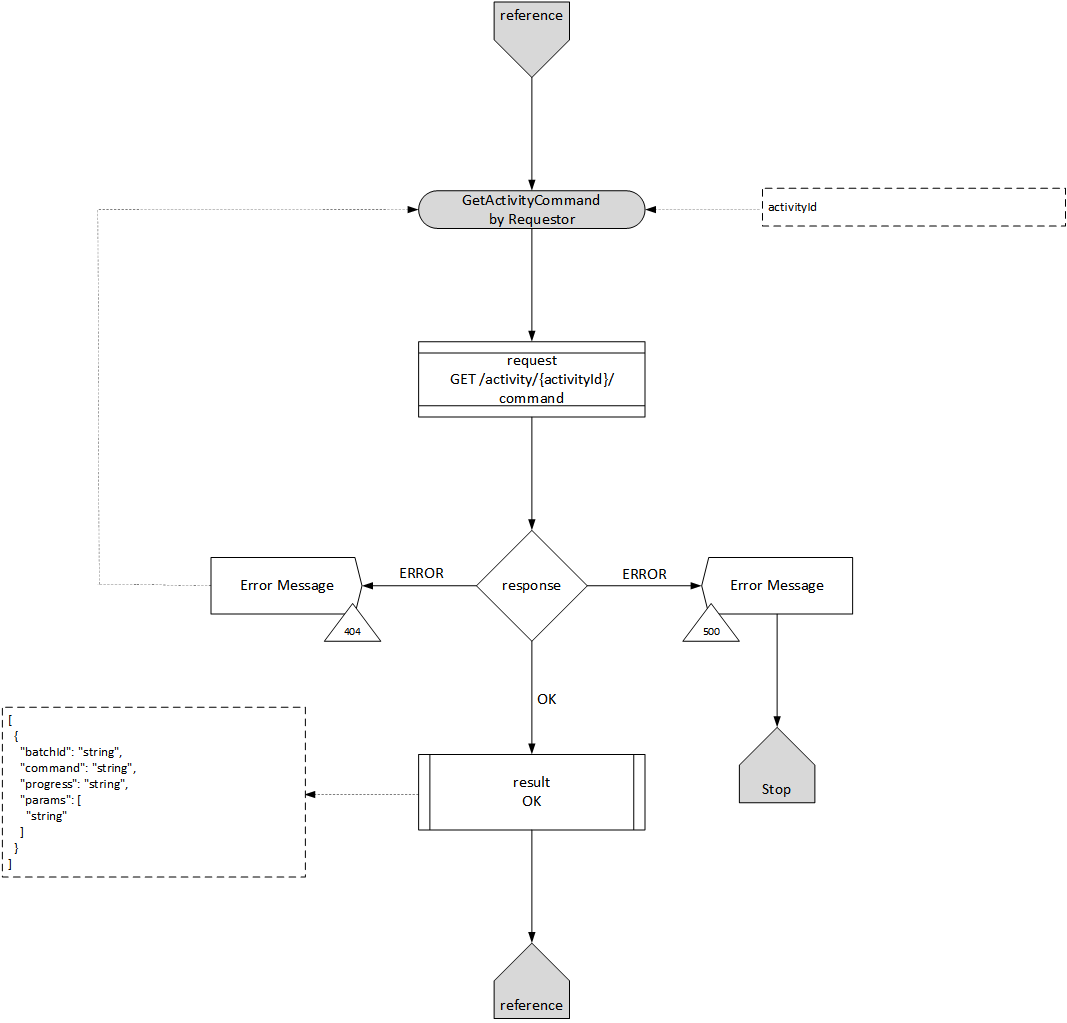
\includegraphics[width=12cm,height=12cm,angle=0]{./diag/Workflow/Activity/GetActivityCommand-R-Workflow.png}
    \caption{Requestor Workflow Get Running Command }
	\label{fig:RGRC}
\end{figure}


\end{enumerate}

\newpage

%% ListenEvent

\subsubsubsection{ListenEvent Function}

\begin{enumerate}

\item Profile

\begin{enumerate}

\item Description

The ListenEvent function is used to return event notifications coresponding to the activity.  
It uses the GET /events method. 

\item Side

Provider

\end{enumerate}

\item Request

\begin{enumerate}

\item Input

\begin{tcolorbox}[boxrule=0pt, frame empty]
\begin{verbatim}

appSessionId
afterTimestamp
timeout
maxEvents

\end{verbatim}
\end{tcolorbox}

%Object

%\begin{tcolorbox}[boxrule=0pt, frame empty]
%\begin{verbatim}

%agreementId

%\end{verbatim}
%\end{tcolorbox}

\begin{table}[H]
\footnotesize

\begin{center}
\begin{tabular}{|p{3cm}|l|p{3cm}|p{3cm}|p{4cm}|} 
\hline
\rowcolor{lightgray}	Name	& MO.	& Type	& Example & 	Description \\
\hline

appSessionId			& O	& 	string				&								& 	A correlation/session identifier used for querying events related to an action 
																						where this appSessionId has been specified	\\ 
\hline

afterTimestamp			& O &	string(\$date-time)	&	YYYY-MM-DDThh:mm:ss.sssZ	&	Apply only to records created later than the specified timestamp \\
\hline

timeout					& O & 	number(\$float)		&	5	&	Timeout used in long-polling calls (in seconds). 
																How many seconds server should wait for response containing new events 
																(0.0 means it should return immediately if there are no events) \\
\hline

maxEvents				& O & 	integer(\$int32)		&	10	&	Maximum number of events that server should return at once. \\
\hline																

\end{tabular}
\end{center}
\end{table}


\item REST Method

\begin{tcolorbox}[boxrule=0pt, frame empty]
\begin{verbatim} 

GET /activity/{activityId}/agreement

\end{verbatim}
\end{tcolorbox}

\end{enumerate}

\item Response

\begin{table}[H]
\footnotesize

\begin{center}
\begin{tabular}{|c|l|} 
\hline
\rowcolor{lightgray}	Code 		& 	Description \\
\hline
200	 		&	OK \\
\hline
403			&	(403) Forbidden	\\
\hline
500			&	(500) Server error. \\
\hline
\end{tabular}
\end{center}
\end{table}

\item Result

\begin{tcolorbox}[boxrule=0pt, frame empty]
\begin{verbatim}

[
  {
    "eventType": "string",
    "eventDate": "YYYY-MM-DDThh:mm:ss.sssZ",
    "activityId": "string",
    "agreementId": "string"
  }
]

\end{verbatim}
\end{tcolorbox}

\begin{table}[H]
\footnotesize
\begin{center}
\begin{tabular}{|p{3cm}|l|p{3cm}|p{3cm}|p{4cm}|} 
\hline
\rowcolor{lightgray}	Name	& MO.	& Type	& Example & 	Description \\
\hline

eventType				&	&	string 				& 								& 		\\
\hline

eventDate				&   &	string(\$date-time)	&	YYYY-MM-DDThh:mm:ss.sssZ	&	Event Date \\
\hline

activityId				&	&	string				&								&	Activity Identifier \\
\hline   

agreementId				&	&	string		&	&	Agreement Identifier \\
\hline  

\end{tabular}
\end{center}
\end{table}

\item Workflow

(Please see Figure ~\ref{fig:PLAE} on page ~\pageref{fig:PLAE}):

\begin{figure}[H]
    \centering
    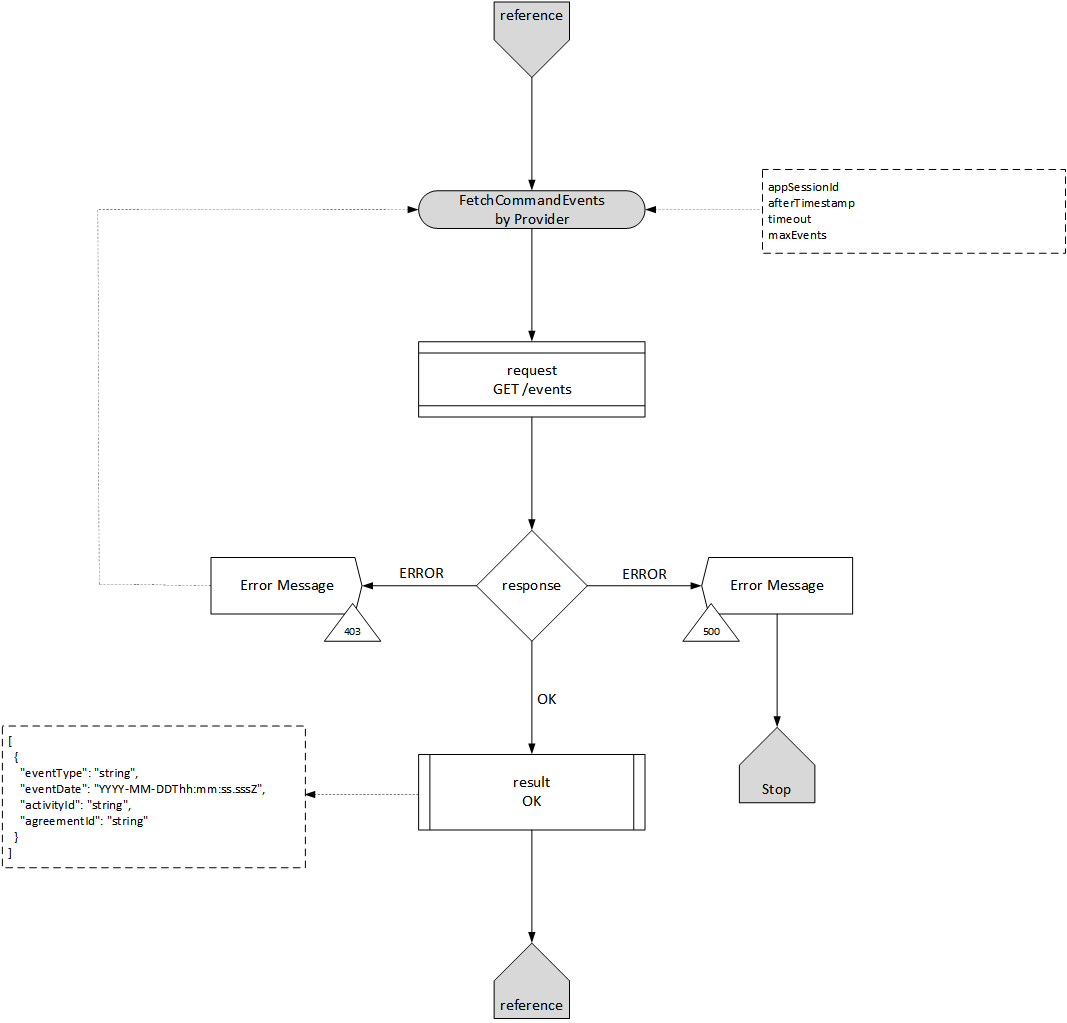
\includegraphics[width=12cm,height=12cm,angle=0]{./diag/Workflow/Activity/FetchCommandEvents-P-Workflow.png}
    \caption{Provider Workflow Listen Activity Event }
	\label{fig:PLAE}
\end{figure}


\end{enumerate}

\newpage